\section{Discussion}
Since the method outlined in this paper did not produce the predicted results and our hypothesis hence remains unproven, a deeper discussion of the apparant failure is of high interest. A correlation between $V_{in} = 5V$ and $V_{out} \approx 5V$ was quickly made, leading to the assumption that some sort of short between $V_{in}$ and $V_{out}$ had occured, the investigation ensued. The thick layer of (non-conducting!) hot-glue, earlier applied as a mechanical safety procedure after repeated pin header related failures, was carefully removed using a flat head screwdriver and rigorous amounts of determination. On closer inspection of the PCB, a short between $V_{in}$ and $V_{out}$ was observed, see Fig.\ref{fig:short}. The reason as to how that short circuit came to be remains unknown. One possible explanation would be that too much solder paste was applied, and the pressure applied during assembly was great enough to smear the paste too far outside the pads, or that it occured during the reflow-phase. A solution to that issue could be to simply use less solder paste, however that raises another issue specific to the Voltera printer; the reliability of the solder paste extrusion suffers greatly on thinner layers, leading to fatal levels of inconsistencies. A better solution would be to extrude the solder paste only on the center of the footprint, instead of printing a solid layer on the whole footprint area. This approach would, as of the current state of the Voltera software, require a custom gerber file with smaller pads used exclusively for the solder paste. A hazzle indeed, but maybe necessary if reliability and repeatability is of any concern.

\begin{figure}[h!]
    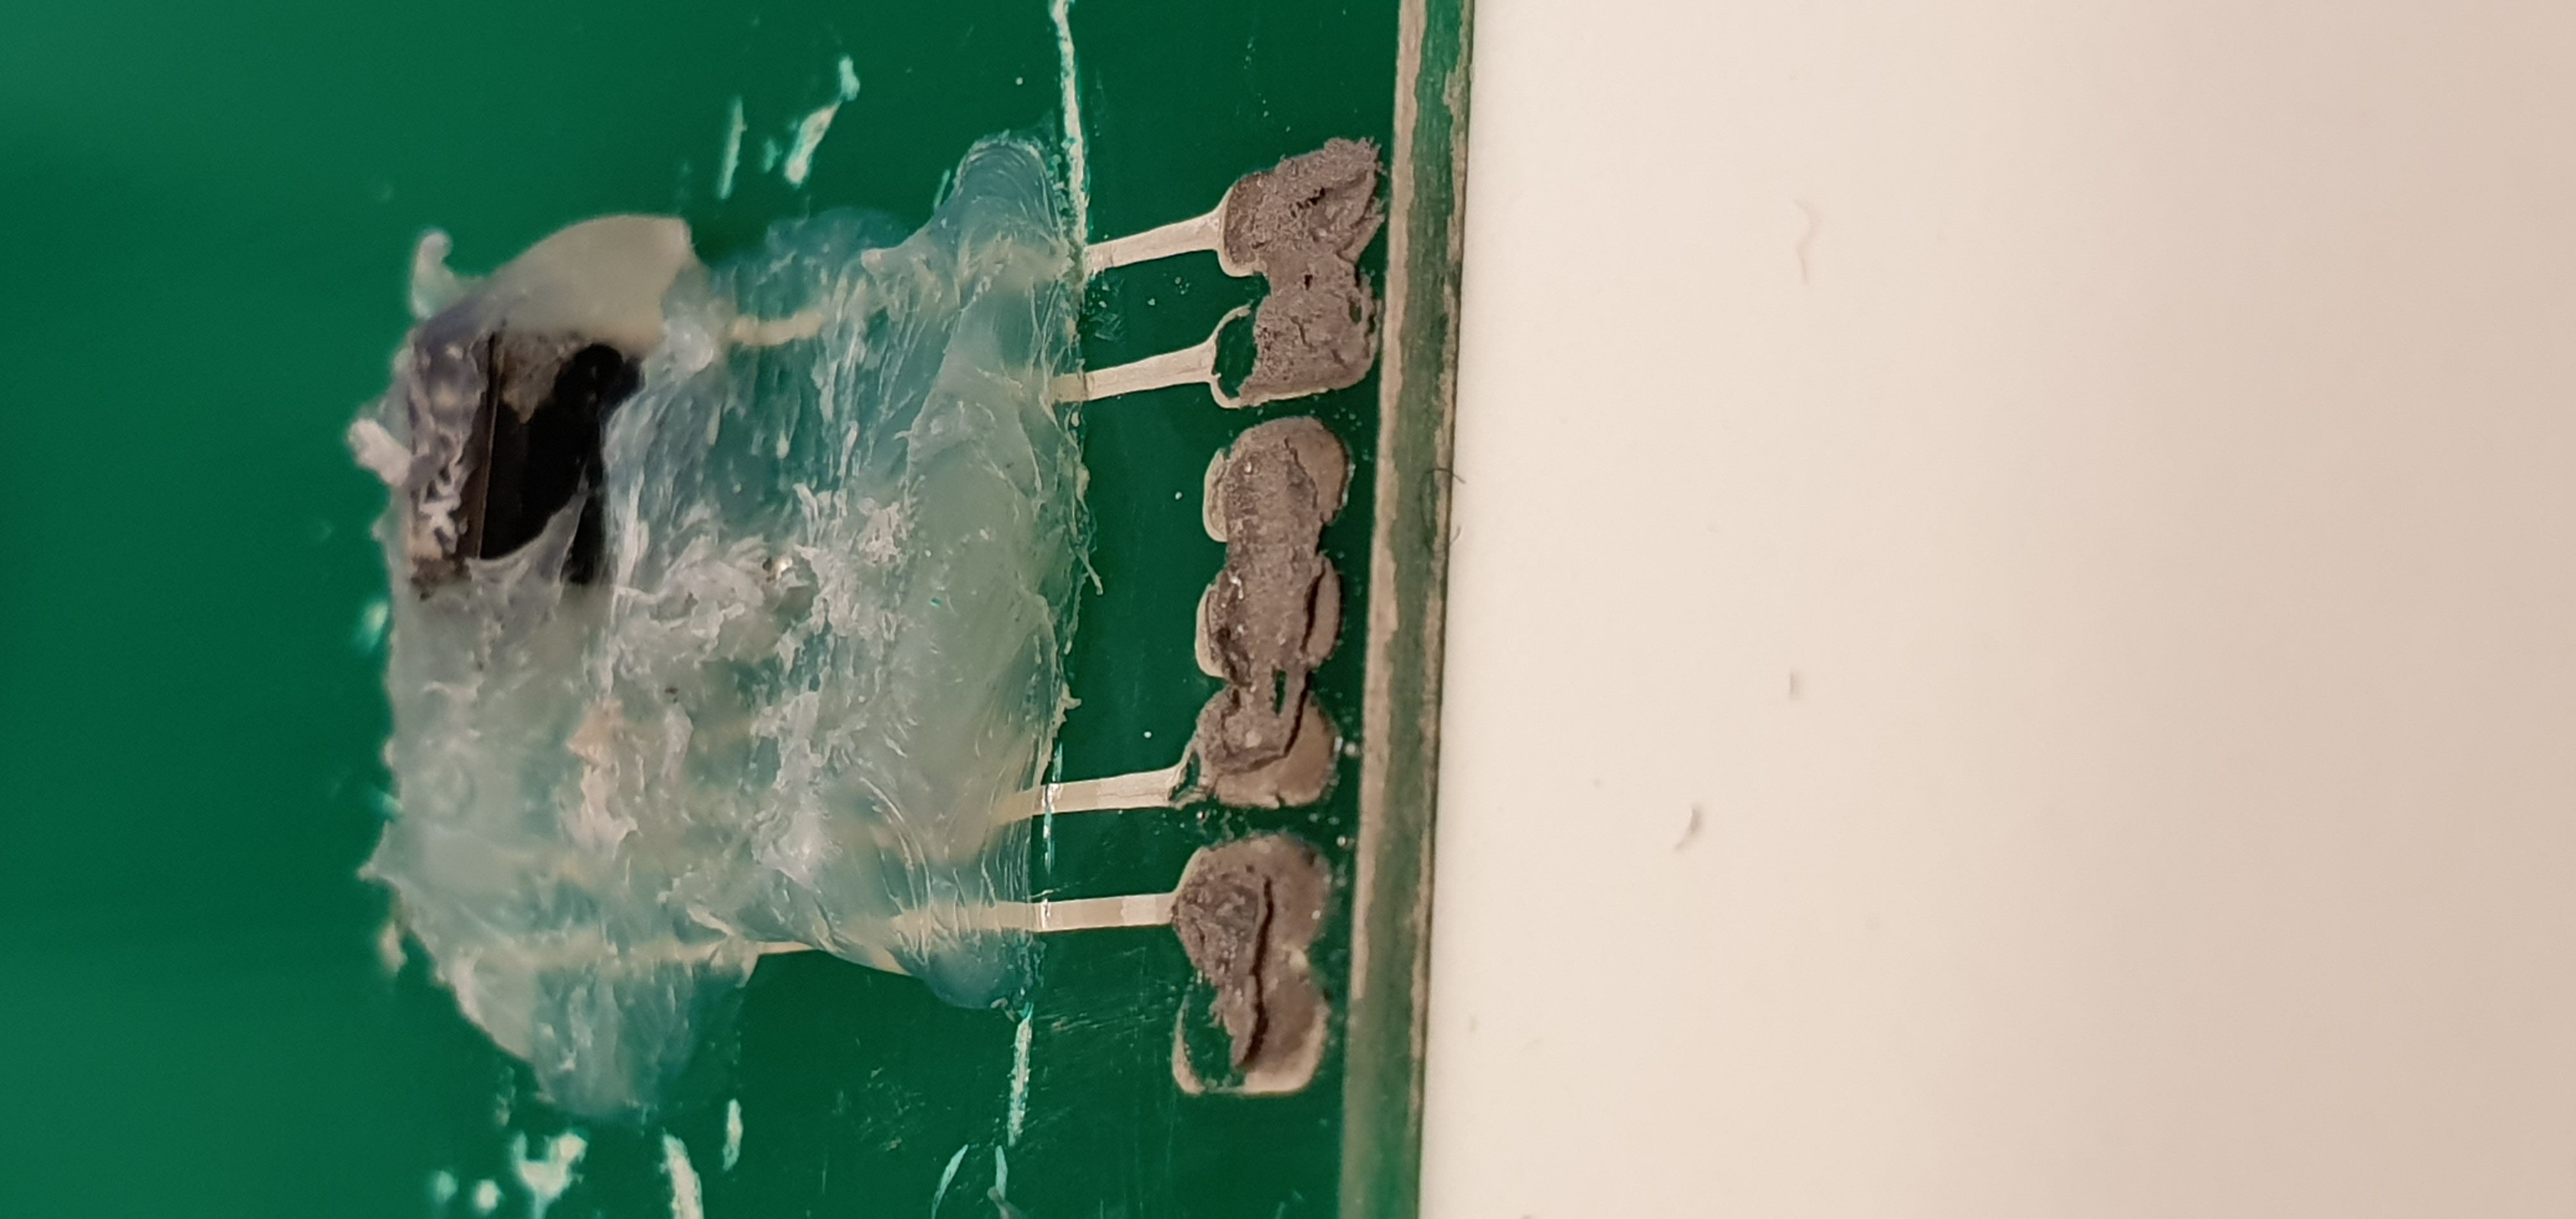
\includegraphics[width=\linewidth]{ela302-kortslutning.jpg}
    \caption{Picture of a short on the pin header. The uppermost pad is $V_{in}$ and the one below is $V_{out}$}
    \label{fig:short}
\end{figure}
